\documentclass[a4paper]{article}
\usepackage{float}
\usepackage{fullpage, amsmath, amssymb, verbatim} % Package to use full page
\usepackage{graphicx}
\usepackage{adjustbox}
\usepackage{url}

\title{Deep Learning: Assignment Three}
\author{Aditi Nair (asn264) and Akash Shah (ass502)}
\date{May 2, 2017}
\begin{document}

\maketitle

\section{Generative Adversarial Networks}

\begin{enumerate}
\item{\textit{Explain generative modeling.} 
\newline
\newline
A generative model uses training data drawn from an unknown distribution $p$, and learns a representation of the distribution, called $\hat{p}$. Generative models can represent $\hat{p}$ directly, generate samples from $\hat{p}$, or both. 

}
\item{\textit{Compare Generative Adversarial Networks (GANs) with other Unsupervised learning approaches, such as Auto-encoders. Explain the difference.}
\newline
\newline
We can compare GANs with other models that estimate probability distributions by choosing distributions that maximize the likelihood of the observed training data. Within this category, we can distinguish between generative models that implicitly and explicitly represent the probability density function $\hat{p}$. 
\newline
\newline
For explicit density models, the maximum likelihood estimation (MLE) task involves choosing probability density functions for $\hat{p}$, and then using gradient descent methods to appropriately parametrize the density functions. Creating MLE-driven generative models that develop explicit density functions are challenging because effectively estimating probability distributions often requires complex models, whose optimization can be computationally intractable. Currently, this is addressed by carefully constructing tractable explicit density functions (like Fully Visible Belief Nets, or FVBNs) and by constructing intractable explicit density functions (like Variational Auto-encoders, or VAEs), which require approximations to complete the MLE task. We will focus on comparing FVBNs, VAEs and GANs since they are currently three of the most popular approaches to generative modeling.
\newline
\newline
FVBNs use the rule of conditional probabilities to represent a distribution $\hat{p} \left( \textbf{x} \right) $ over an $n$-dimensional vector $\textbf{x}$:
$$\hat{p} \left( \textbf{x} \right) = \prod_{i=1}^n \hat{p} \left( x_i | x_1,...x_{i-1} \right) $$
That is, the probability distribution over $\textbf{x}$ is defined as the product of the conditional probabilities over its individual components. In particular, this operation cannot be parallelized because of the conditional nature of the computation. In WaveNet, a popular approach to FVBNs, each $\hat{p} \left( x_i | x_1,...x_{i-1} \right)$ is computed by a neural network. Accordingly, the computation of each conditional probability can be expensive, and can only be executed sequentially, making it difficult to scale the model for more demanding tasks. 
\newline
\newline
Next, we consider VAEs, which fall in the category of explicit density models which rely on approximation to complete the MLE task. Intuitively, VAEs use encoders to transform high-dimensional input vectors $x$ into a lower-dimensional latent space representations $z$, and then attempt to re-construct the original vectors using decoder networks. Probabilistically, we can argue that we would like to calculate the posterior distribution $p \left(z|x \right) $ so that we have good estimates for $z$ given the training data $x$. In variational inference, we approximate this distribution with $\hat{p} \left( z|x \right)$. In order to optimize our choice of $ \hat{p} \left(z|x \right)$ we would like to minimize the Kullback-Leibler divergence:
$$KL\left( \hat{p} \left(z|x \right) |  p \left( z|x \right) \right)  = \int_{x} \hat{p}(z|x) log \frac{\hat{p}(x|z) }{p(z|x ) } $$
$$ = \int_{x} \hat{p}(z| x) log \ \hat{p}(z |x)  - \hat{p}(z| x) log \ p(z|x )  $$
$$ = \mathrm{E}_{\hat{p}} [ log \  \hat{p}(z |x) ] - \mathrm{E}_{\hat{p}} [ log \ p (z | x) ]  $$
By Bayes' Rule:
$$ p (z|x) = \frac{p(x,z)}{p(x)}$$
So we can write:
$$KL\left( \hat{p} \left(z|x \right) |  p \left( z|x \right) \right) = \mathrm{E}_{\hat{p}} [ log \  \hat{p}(z |x) ] - \mathrm{E}_{\hat{p}} \Big[ log \ \frac{p(x,z)}{p(x)} \Big] $$
$$ =   \mathrm{E}_{\hat{p}} [ log\  \hat{p}(z |x) ] - \mathrm{E}_{\hat{p}} [ log \ p(x,z) ] + log \ p(x)$$
Clearly the term $log \ p(x)$ is intractable. Either we must know the distribution $p(x)$ - in which case we have already solved the problem of generative modeling - or we must compute it by marginalizing over $z$ - $\int_z p(x|z) p(z) dz$ - which is intractable since the space of all possible $z$ is large. However, we observe that by maximizing the following tractable expression:
$$\mathrm{E}_{\hat{p}} [ log \ p(x,z) ] - \mathrm{E}_{\hat{p}} [ log\  \hat{p}(z |x) ] $$
we minimize the KL-divergence as written above. Therefore, in the VAE setting, we choose to maximize the above expression, known as ELBO, instead. However, optimizing over the ELBO only provides a lower bound over the original KL-divergence, which has an added $log \ p(x)$ term. In addition, if we choose an inappropriate distribution for the prior or the posterior of $\hat{p}$, then we end up selecting $\hat{p}$ poorly. This is the primary weakness of VAE models, in addition to the lower quality of their generated samples.
\newline
\newline
Finally, we consider GANs. A GAN can be described as a game between two adversarial players, a generator $G$ with parameters $\theta^G$ and a discriminator $D$ with parameters $\theta^D$. The generator creates samples which appear to be drawn from original distribution $p$. The discriminator classifies samples as being real (drawn from the original distribution) or fake (created by the generator), and is trained to minimize the following loss:
$$ J^D(\theta^D, \theta^G) = -\frac{1}{2} \mathrm{E}_{x \sim p_{data}} [log\ D(x)] - \frac{1}{2} \mathrm{E}_z [log\ (1 - D(G(z)))]$$
The first summand expresses the cross-entropy loss of the discriminator on real samples drawn from the training data. $D(x)$ expresses the discriminator's probability estimate that $x$ is sampled from the data. If $D(x) = 1$, then $log\ D(x) = 0$ and the left summand is minimized. The second summand expresses the cross-entropy loss of the discriminator on ``fake" samples created by the generator. $z$ are noise vectors sampled from a prior distribution (e.g. a uniform distribution on a unit hyper-cube), which are fed to $G$ to create fake samples. $D(G(z))$ expresses the probability that $z$ is sampled from the data distribution, so $1- D(G(z))$ expresses the probability that $z$ is fake. If $D(G(z)) = 0$, then the discriminator is certain that a fake is indeed fake, and the right summand is minimized. Note that $ J^D(\theta^D, \theta^G)$ is a function of $\theta^D$ and $\theta^G$, but $D$ can only optimize over $\theta^D$.
\newline
\newline
Next, the generator is trained to ``fool" the discriminator. The loss function used for the generator can vary, but a common one is the cross-entropy loss:
$$J^G(\theta^G, \theta^D) = -\frac{1}{2} \mathrm{E}_z [log \ D(G(z))] $$
$J^G$ is a function of $\theta^D$ and $\theta^G$ but $G$ can only optimize over $\theta^G$. If $G(z)$ looks exactly like a sample drawn from $p_{data}$, then $D(G(z)) = 1$ and we will minimize $J^G$.
\newline
\newline
Typically, both the generator and the discriminator are neural networks which are trained simultaneously using gradient descent on real and fake samples. Unlike FVBNs and VAEs, GANs only provide us with an implicit representation of $\hat{p}$, since the generator is a neural network constructed to create the $G(z)$ samples. For the same reason, unlike FVBNs, GANs can generate an entire sample simultaneously. Whereas VAEs require you to carefully select the distribution for the approximator $\hat{p}$, the neural networks used in GANs are generally considered universal approximators. In addition, unlike (most) VAEs, a GAN trained with sufficient data can theoretically recover the true distribution $p_{data}$ - it is clear above that both $J^G$ and $J^D$ can be minimized directly, whereas we can only minimize the ELBO of the VAE loss function. Finally, it is worth noting that GANs are (subjectively) considered to produce better samples than VAEs and FVBNs.

\begin{comment}
Credit https://jaan.io/what-is-variational-autoencoder-vae-tutorial/ for VAE explanation
\end{comment}
}
\item{\textit{Explain conditional generation using GANs, versus the vanilla unconditional version. Please briefly draw a diagram when training conditional GANs, with the condition context C, generator G, discriminator D, random vector z and output x.}
\newline
\newline
In the previous presentation of GANs, we described ``vanilla" unconditional generation where we take $z$ samples from a noisy prior distribution and feed them into the generator $G$. One problem is that we have no control over the kind of sample we generate - or, mathematically speaking, on the distribution of the samples being generated. 
\newline
\newline
To address this issue, Mirza and Osindero (2014) suggest building Conditional GANs, which condition both the generator and discriminator on some context $C$. For example, Mirza and Osindero set $C$ as one-hot vectors indicating class labels for data.
\newline
\newline
In the generator, we combine the noise vector $z$ with the context $C$ at the input layer (for example, by concatenation), before feeding it through an appropriately-sized convolutional network to generate $G(z|C)$. Ideally, $G(z|C)$ should look like it belongs to the class of $C$. In the discriminator, we similarly combine the inputs $X$ (either $G(z|C)$ or $x \sim p_{data}$) with the appropriate one-hot vector $C$ before feeding it through an appropriately-sized convolutional network to compute $D(X|C)$. Finally, to generate samples of a specific class, we simply sample $z$ from the noise prior, concatenate with the $C$ vector for the intended class and compute $G(z|C)$. 
\newline
\newline
Below, we provide a diagram of the Conditional GAN framework (borrowed from Mirza and Osindero and modified with our notation):
\begin{figure}[H]
  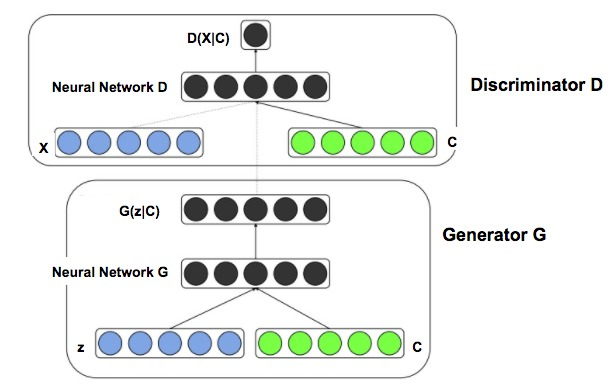
\includegraphics[scale=3]{images/my_conditional_gan.jpg}
  \label{fig:boat1}
\end{figure}

\begin{comment}
Cite: Mirza and Osindero "Conditional Generative Adversarial Networks" (2014)
\end{comment}

}
\end{enumerate}

\section{GAN Workhouse}

\subsection{MNIST}
To begin our exploration of GANs, we decided to build off of the work done by Radford et al. in their creation of the DCGAN model. Due to the generally strong performance of the DCGAN model across a variety of generative tasks for images, we decided that it would be a good starting point. We started by using the DCGAN model on the MNIST dataset of 60,000 images, without labels, for a vanilla GAN task. Since DCGAN is such a powerful and deep GAN model, we found that it trained very easily on the MNIST dataset. Even after only 10 epochs, we found the generated output to be quite reasonable and expected that by running the model for longer we could have high quality generated images for hand-written digits. A sample of the generated output after only 10 epochs is shown below:

\subsection{CIFAR-10}
In order to take on a more challenging task, we decided try training GANs on the CIFAR-10 dataset\footnote{\url{https://www.cs.toronto.edu/~kriz/cifar.html}}. The CIFAR-10 dataset consists of a set of images with 10 classes: \{airplane, automobile, bird, cat, deer, dog, frog, horse, ship, truck\}, and the images are "tiny" so we found that the resolution quality of the images is not very good. We started by training the original DCGAN model on this dataset. Generated output of the model after 40 epochs is shown below:

We wanted to incorporate the conditional GAN framework outlined in Conditional Generative Adversarial Nets\footnote{\url{https://arxiv.org/pdf/1411.1784.pdf}} into the DCGAN model, so that we could try utilizing the class information while training on the CIFAR-10 dataset. This would also allow us to do class-conditioned generation of images. As described in the paper, a vanilla GAN can be extended to a conditional GAN by feeding additional information, which could be class labels or data from other modalities, into both the generator and the discriminator. 
\\\\
In the first version of our conditional DCGAN model, we concatenated the input noise vector for the generator and a randomly chosen one-hot encoding of a class label, then passed this entire concatenated vector into the generator. Other than that, the architecture of the generator was exactly as before in the original DCGAN model. The first part of the discriminator worked as before, where an image tensor that came from either a real example in the data or from the generator would be passed through a series of convolution, leaky ReLU, and batch-norm layers. However, after the final convolution layer when we had a single feature vector as the output, this feature vector was concatenated with a one-hot encoding of a class label. If this image being passed through the generator was from the dataset, then its true class label would be used, while if the image was generated by the generator then the class label used for its generation was used. The concatenated vector of the feature vector and the one-hot labels would then be passed through a sigmoid layer, consisting of an affine transformation mapping the input vector to a single output and then a sigmoid non-linearity giving us a probability. 
\\\\
In this model, we now have a new parameter that can be tuned - the dimension of the convolution feature vector in the discriminator that is concatenated with the one-hot labels. We experimented with dimensions of 100, 200, and 400. We found that the dimension of 100 resulted in the lowest quality images, while 200 and 400 were more similar but 400 was slightly better. We concluded that more expressive features from the convolution resulted in better performance in the model. Below we show output from our conditional model with a convolution feature vector dimension of 400, trained for X epochs:
\\\\
When using the model to generate class-conditioned images, we tried feeding in batches of the same fixed noise vector with each of the class labels to see if the model generated appropriate images for each class. However, we noticed that all of the images with the same fixed noise vector were very similar, even though they had different class labels, as shown below:
\\\\
This motivated our attempt to modify the architecture so that the model put more weight on the class labels in the discriminator and the generator. We thought one issue might be that the magnitude of the values in the feature vector produced by the convolution layers of the discriminator might be much larger than the values of the one-hot encoding vector, which are 9 zeros and 1 one. Our attempt to fix this was to add a batch-normalization layer to this feature vector before it is concatenated with the one-hot encoding vector. However, this did not work well at all and the images produced resembled pure noise. We realized that rather than simply using the one-hot encoded vector, it might improve the model to learn an embedding on this vector. Thus, we added a sigmoid layer to the generator which affine transformed the one-hot encoded vector into a 200 dimensional vector and then applied a sigmoid non-linearity. The rest of the network was the same as before, as this 200 dimensional vector was concatenated with the noise vector and passed through a series of convolutional layers to generate an image. We similarly added a sigmoid layer in the discriminator which again transformed the one-hot encoded vector into a 200 dimension vector, before concatenating it with the convolution feature vector and passing the concatenated vector through the final sigmoid layer to get a probability output. Below, we show some generated images from this version:
\\\\
In comparing the quality of our generated images and the number of epochs run to work done in Conditional Generative Adversarial Nets for Convolutional Face Generation\footnote{\url{http://www.foldl.me/uploads/2015/conditional-gans-face-generation/paper.pdf}}, we noticed that it took approximately 130 epochs of training to obtain high quality generated face images, while between epochs 60 and 80, the generated images had some local qualities of faces such as color patterns and borders but not strong global resemblance to faces. Due to computational resources, we were able to train many of our models in the range of 40 to 60 epochs, and as in the paper, we noticed that our generated images had some local qualities that resembled images from the original data. However, we suspect more training time is needed to get high-quality generated images. Furthermore, the low resolution quality of the original images negatively impacted the quality of our generated images. We did not train our models with GPUs, but we expect that utilizing GPUs would likely have allowed some of our models to train past 100 epochs where we could expect higher quality generated images. 


\end{document}
